\documentclass[11pt,a4paper]{article}
\usepackage[latin1]{inputenc}
\usepackage[pdftex]{graphicx,color}  
\usepackage[linkcolor=blue, colorlinks=true]{hyperref}
\usepackage{multicol}
\usepackage{titlesec}

\setlength{\hoffset}{0pt}
\setlength{\voffset}{0pt}
\setlength{\oddsidemargin}{0pt}
\setlength{\topmargin}{0pt}
\setlength{\headheight}{0pt}
\setlength{\headsep}{0pt}
\setlength{\textheight}{\paperheight}
\addtolength{\textheight}{-2.2in}
\setlength{\parindent}{0cm}
\setlength{\parskip}{.2cm}
\setlength{\tabcolsep}{.2cm}
\setlength{\textwidth}{\paperwidth}
\addtolength{\textwidth}{-2in}
\clubpenalty = 10000
\widowpenalty = 10000 
\displaywidowpenalty = 10000

\titlespacing\section{0pt}{6pt plus 2pt minus 1pt}{1pt plus 1pt minus 1pt}

\titleformat{\section}{\normalfont\fontsize{12}{15}\bfseries}{\thesection}{1em}{}

% XXX also shrink section sizes slightly

\pdfinfo {            
	/Title(Stable, Composable and Efficient Paging of Result Sets)
}

\title{Stable, Composable and Efficient Paging\\ of Result Sets}
\author{Robert Lemmen $<$robertle@semistable.com$>$}
\date{\today}

\begin{document}
\maketitle
\bigskip

\begin{abstract}
\noindent Paging of results sets, showing a limited section of the results with
the ability to navigate to the adjacent sections, is a common and seemingly
trivial method used in computer systems. As usual, the devil is in the details
however. A simple and widespread approach is to use an offset into the result
set. This text shows problems resulting from this strategy, how they can be
overcome with a small modification, and how this can be leveraged to solve
even more interesting problems.
\end{abstract}
\vspace{40pt}

\begin{multicols}{2}
\section*{A Paging Example}
In order to illustrate the next sections, it is useful to have a common and
simple example case. Suppose we have a computer system containing a set of
records and making these records available to the user. We only want to present
a limited set of records with a given size to the user at a time, and the user 
should be able to retrieve the next set, or go back to the previous set. A very
common setup that we are all familiar with.

In our example the records will initially only be simple numbers. Not a very
useful system, but sufficient for this discussion. Our system will contain only
the numbers 2, 4, 5, 6, 8, 10, 11, 12, 14, 16, 17, 18, 19, 21, 24, 26. We will
also fix the size of a result set page to 5. We will allow a set of retrieval
options like filtering, search and ordering as we expand the example, but
initially the number are always presented in their natural numerical order, and
all numbers are returned. 

So the if the user submits a query, the first page presented should contain the
numbers 2, 4, 5, 6, and 8, and the next page 10, 11, 12, 14, 16. Overall there
will be four pages, with the last on consisting of only one element, 26. 

\section*{Using Offsets}
The most common approach to implementing this is using an offset into the full
result set. So for example a function would be invoked with query parameters
like ordering and filtering predicates, and an initial offset = 5 and a
pagesize of 5. The implementation of this function would somehow apply the
ordering and filtering, and then returnd the items starting with the element at
position {\em offset} in the list, stopping after it has returned {\em
pagesize}. 


\includegraphics{offsets.pdf}

When the user navigates to the next page, the presentation logic simply adds the
pagesize to the current offset, yielding the offset of the next page and uses
this for the next query. In the same way, the previous page can be addressed by
subtracting the pagesize from the current offset. 

\section*{Stability}
It is interesting to observe what happens when we modify the data in our system
between two calls that present adjacent pages. There is no ``transactionality''
over the two page presentations, so we cannot expect to see an isolated full
view of either the old or the new state. In other words if an item gets added to
the list then we might or might not see it when paging through the result set,
depending on when it was added relative to the flip from one page to the next,
and depending on which page it is on. 

What we do not expect however, is that the addition or removal of an item has an
effect on the visibility of other items. Unfortunately this is the case however. 

In our example we have just retrieved the first page (2, 4, 5, 6, 8), when the
number 6 gets deleted from the system. If we were to re-retrieve the first page
at this point, we would get 2, 4, 5, 8 and 10 instead. But we do retrieve the
second page, unaware of the modification, and get 11, 12, 14, 16, and 17. So the
removal of item 6 has led to the fact that we have seen 6, but have
missed 10 instead. In a similar effect, the addition of items in a page before
the one we are currently looking at will lead to items being present on multiple
pages. This effect gets worse with the size of the result set, as addition or
removal of items affects all following pages. The bigger the result set, the
more pages are affected by a change.

\section*{Efficiency}
Earlier we said the implementation of our query method would return items 
``...starting with the element at position {\em offset}...''. This is worth
examining: while some data structures that could potentially be used to hold our
data do support direct and efficient addressing of elements by their position
(e.g. arrays), these are unlikely to be used for any real-world application.
Much more likely are search trees of some sort or other data structure that 
allow efficient ($\mathcal{O}(\log{}n)$ or better) search and insertion. In 
these, the only way to locate an element by a
given position is to iterate from the start to that position and simply discard
all elements prior to the desired one, a $\mathcal{O}(n)$ operation. There are
no data structures that allow all three operations of insertion, search and
direct addressing by position efficiently. 

Even if there was a data structure that would support this, it could not
continue to work in the presence of a filtering predicate. If for example we
instruct our system to only return even numbers, it would have to iterate
through the items in our database, check for each of them whether it is even or
not, and keep count of how many fulfill this criteria, before it could determine
where the start of the new page is.

The fact that finding a single page has a complexity of $\mathcal{O}(n)$ is bad
enough, but it also means that traversing all pages has a complexity of
$\mathcal{O}(n^2)$, always a sign of trouble.

Note that the complexity of this is often hidden, which of course does not make
it go away. For example many SQL servers implement an OFFSET query parameter
which allows a simple implementation of this type of paging. Inspection of the 
quer plan however reveals that the implementation of this is just as described above:
linear scan over the result set, just not returning any data until OFFSET is
reached.

\section*{Simple Locators}

Fundamentally the problem with the offset is what it is relative to: the start
of the result set, which can be pretty far away and requires understanding of
everything inbetween. The alternative is to use something much closer to the
current page, a virtual item that sorts just before the start of the page under
some ordering predicate: a {\em locator}. If we have such a locator, we can provide it
to a query instead of an offset, and in our (or the database implementation) we
can use it to quickly locate the start of the page by comparing in a binary chop
or tree traversal.

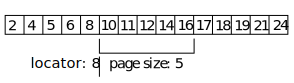
\includegraphics{locators.pdf}

This sounds a little bit abstract, but in a simple concrete case it is rather
trivial: in our number server from above, the type of the locator could also be
a number. Note that it is the same type, not necessarily one of the numbers in
our database. For example we would query our server with a locator value of 8,
and a page size of 5 as above. Internally we would use a $>$ operator as the
ordering predicate. If our implementation uses a binary chop, it would take
$\mathcal{O}(\log{}n)$ comparisons to find out that the first item greater than
the locator is 10. Note that this uses a
strict ordering between locators and items, which is counter-intuitive but
important. It may help to think of them as different types despite the obvious
similarily in this simple example. So our page would start with the first item
for which the ordering predicate no longer returns true. If the implementation
uses a more clever search strategy, e.g. a btree or so, the time complexity
stays the same of course.

Note that this also works for the very first element, e.g. if we supply a 0 as
the locator. This requires a value for the locator type that is considered less
than the smallest possible actual entry in the database, something that
typically requires some work in the form of a special value, a nullable locator,
or a composite locator that has an extra attribute marking it as the beginning.

Also note that the effort of locating the start of the page is the same across
the whole result set, no matter how large it is. This addresses the efficiency
problems of the offset approach, leading to a complexity for iterating the whole
result set of $\mathcal{O}(n\log{}n)$.

A key difference between the two approaches however is that in the offset case,
the client can compute the offset of the next page just based on the query
parameters used for the current one. In the locator case the server needs to
provide a locator for the next page along with the page contents. This may seem
redundant in this simple example, because the locator for the next page could
just be the last entry of the page. But remember that the locator and the item 
are technically different types, and in more complex cases they will also be
different in practice. Therefore it is very important that clients do not
attempt to construct, compose or otherwise interpret locators. They should just
treat them as opaque ``handles'' that are passed back to the server.

The locator is typically derived from the last element of the current page. 
This has the drawback that if that is the last element in the whole result set,
the client would retrieve the next page using that locator, which then turns out to be empty. A way to
mitigate this is to always retrieve one item more than the page size, but not
return it to the client. If that item does not exists, the locator is set to a
special ``end'' value (which could be the same as the ``start'' one used by the
client). Whether this optimization is worth the extra complexity depends on the
use case, e.g. for a user-facing system an empty last page could be confusing
and frustrating, if the client is another computer system then it is probably
used to that type of frustration already..

\section*{Locator Stability}

Despite the warning to not invent locators on the client side, it is interesting 
to see what would happen when using a locator that was not previously returned as part of a page. For example 
if we use 9: the locator value is different, but it would still be ordered in the same
place, between 8 and 10, and consequently the page returned is exactly the same.
This also works the other way around: if the locator stays the same, but the
result set changes because items are added or removed, the page returned is not
affected as long as the items added/removed are on this page. So the locator
stability problem of the offsert approach is fixed too.

Even if the page in question is affected, the results are hard to distinguish
from the case where the modification happened just before or after the page
retrieval. For example if the locator is 10, but 10 got removed between the two
page retrievals. The final full result set and the division into pages is just
the same as if the retrieval happened after the removal. The only difference is
the locator used at some point, but we already established that the client is
not meant to look at the locator too closely.

\section*{Locating Backwards}

Of course clients may also navigate backwards sometimes, which is more
complicated than in the offset case. First of all it ideally uses a different
locator, one related to the start of the page and derived from the first
element. It also requires a flag by the client that indicates whether we are
paging forward or backwards from the locatodirect page access. Based on this the
implementation would reverse both the ordering when iterating the result set, as
well as use a different ordering predicate. Interestingly the reverse ordering
predicate cannot be constructed from the forward ordering predicate by inversion
as that would turn $>$ into $<=$, which is no longer a strict ordering. In many
cases the reverse ordering predicate can however be constructed from the forward
ordering predicate by inversion of the paramters (of course).

In most cases it makes sense to reverse the
order of the items returned again before returning them to the client. That
can also be done on the client before presenting them of course, but it would
mean the client needs extra logic and also needs to keep track of whether it has
retrieved the page in forward or backwards mode, which may require extra state.
If the server always presents the page in the natural or requested order, then
the client can be stateless and can derive the requests for the previous or next
page from the current result page including the locators provided.

\includegraphics{locate-back.pdf}

\section*{Transformations and Filtering}

An interesting property of locator-based paging is that functionality can be
built that builds on top of a paging access, provides a paging access, yet adds
extra value.

One simple example is an enrichment of the data provided. It is relatively
straight-forward to, when asked for a page of results, go to some other system
and request a page of raw data, and then apply a function to each element. This
could be a transformation, mapping, or requesting extra data per item and
enriching the page. This is already possible of course with offset-based
paging.

Very often however the transformations required are more structural in nature
and will either filter out some items, collapse adjacent items together or even
split an item into multiple ones. This is not possible with offset-based paging
as changing the number of items of course affects the offset of all subsequent
items, and therefore means breaking the relationship between the incoming page
request being handled, and the request or requests that need to be done to the
upstream backend.

% XXX filtering example with image

What is not possible of course is changing the order of items in the virtual
total result set, or operations that collapse two non-adjacent items. That
however is the same for offset-base paging.

\section*{Composing Locators}

A slightly more advanced method of building pages based on other pages is to
create a singler page from multiple pages from different sources. This is
possible because our locator is an opaque piece of data and might well contain a
structure of multiple data points. This is not possible with offset-based
locators, and is highly interesting because it allows locating data in different
places that otherwise would have to be colocated just for the technicality of
the access patterns. In other words it enables federated or distributed systems.

As an example, we could decide to shard our extremely large collection of 16
numbers over two systems for scalability reasons. One of our systems would
contain even numbers, the other odd ones. The composability described
below does not depend on the criteria used to distribute the data, so in reality
a little bit more useful criteria could be used.

The aggregation service would receive a request like in the example above, with
a page size of 5 and a locator value of 8. Since the two sources have the same
structure, it can simply pass on the request to both of them. It would then have
to combine the two results, sort them, and discard the unnecessary items. 

\includegraphics{composing.pdf}

In this case the locator used in all three cases is exactly the same. This is
possible in many cases, especially when the structure of the data from all
upstream sources is the same. It is not required however: the aggregating
service could simply use a tuple of all upstream locators to the client. In the
example above the locator for the next page could e.g. be expressed as
``16;11''. Structured or multi-value locators do require a little bit more
serialization effort for them to be safe to transport over the wire.

The example also shows that this composition of pages has to discard some
fetched items, which is a bit wasteful. An alternative would be to request
pages from the upstream sources that are smaller than the requested page, and
make subsequent calls if this turns out to not provide enought data. This is a
tradeoff informed by the number of upstream sources, page sizes, uniformity of
data distribution and relative cost of larger pages versus extra calls. In most
cases the simple approach of simply requesting a full-szied page from each
upstream source is the best.

Combining multiple source pages requires the aggregating service to order them
again, which in turn means it needs to fully understand the ordering predicate
used by the sources. This needs to be taken into account as it presents an
element of coupling. On the other hand the ordering predicate is typically a
high-level requirement of the total system behavior, rather than some
technicality so this coupling may not be so tragic.

Up to this point it would have been tempting to represent a page of results as
an array of items together with a forward and a backwards locator. Note however
that due to the discarded elements, this is not enough to build composable
pages. A better and simpler, albeit slighly more wasteful, approach is to
provide a locator for each item in the result page, and to ensure that a locator
can be used as both a forward and a backwards locator (as in all examples
here).

% XXX direct page access and page count

% XXX building offset-based paging on top of locators

\section*{Timestamps as Locators}
If you have locators, everything looks like a page! There are plenty of
interesting access patterns that can also be viewed as paging, when picking the
right ordering predicate. Assume for a moment we have a service holding records
of some sort, each with a unique Id as well as a last-modified timestamp. This
data is required in other places and joined with other data, transformed or
indexed there (event sourcing, materialized views\ldots). When a new system
requiring the data starts up, it needs to fetch all data. This may be a lot, so
some sort of paging is required. Subsequently, it needs to refresh the local
cache, a delta update based on the last-modified timestamp. The amount of data
changed since the last interaction is also pretty much unbound and therefore
requires pagination. Paging through the data changed since some point of time
in an offset-based approach can lead to missed updates if the data changes again
however (see above), and generally requires extra state to be able to keep the
resultset currently being traversed stable while paging through it. 

Locators allow all of these access patterns to be implemented in the same way:
The data source would simply expose a locator-based retrieval mechanism with an
ordering predicate that sorts by last-modifed first and ID second. The locator 
would therefore be a tuble of both values. In some case of more complicated
timestamps, like thos used in distributed systems, the timestamp is unique and
the secondary ID ordering is nort required. 

With this setup, the initial fetch is the same as subsequent updates: simply
keep paging until the end of the resultset from your current locator, which may
be a conceptual zero locator on startup. Note that once you have reached the end
of the result set, you may still discover more data there later. In a way it is
an infinite, lazy result set that the client is paging over.

\section*{Summary}
% XXX 

\end{multicols}
\end{document}
